%************************************************
\chapter{Theoretical Background }\label{theory} % $\mathbb{ZNR}$
%************************************************

%And is it over now, do you know how
%Pickup the pieces and go home.
%Fleetwood Mac, \textit{Rumours}, 1977
%Press your space face close to mine, love
%\begin{flushright}{\slshape    
%	I think, I'm looking on the dark side \\
%	But everyday you hurt my pride \\
%	I'm over my head \\
%	Oh, but it sure feels nice} \\ \medskip
%    --- {Fleetwood Mac, \textit{Over My Head}, 1975}
%\end{flushright}

\section{A Little History}
Our understanding of the universe develops in a leap-frog of theory and observation, one catching up to and surpassing the other as technology improves, to be passed in turn by a new idea or new observation. The picture of dark matter commonly accepted today is much different than what Zwicky anticipated in 1933 when he found that the velocity dispersion of the galaxies in the Coma Cluster was much larger than expected from the Virial Theorem \cite{Zwicky1933}. This observation is typically cited as popularizing the term ``dark matter'', and starting the hunt for the mysterious invisible substance. Zwicky postulated that the faster rotation was caused by dark matter consisting of cold gas or stars and both macro- and micro-scopic solid bodies, and estimated that there was about 400 times more dark matter than visible matter. Smith, a contemporary of Zwicky's, did a similar analysis with the Virgo Cluster and his results yielded a much smaller dark matter to visible matter ratio \cite{Bertone2016}. Meanwhile, many in the astrophysics community disagreed with an underlying assumption of these analyses and argued that galaxy clusters are not at equilibrium so the Virial Theorem does not apply \cite{Bertone2016}. At the time, the only consensus reached was that more information was needed to understand the dynamics of galaxy clusters. 

In the 1970's, a new technology called the image tube spectrograph allowed Vera Rubin and Kent Ford, the developer of the spectrograph, to measure the rotational velocity of the Andromeda Galaxy at different points along its radius (called a galactic rotation curve) \cite{Rubin1970}. The new data was of higher quality than previous attempts at measuring galactic rotation curves, and the result, that the galaxy was rotating faster than expected at large radius, indicating ``hidden mass'', was soon replicated by others \cite{Bertone2016}. Over the next decade, a significant number of galactic rotation curves were obtained, all showing essentially the same result: galaxies were rotating faster than expected at high radii, indicating that the mass of galaxies continued to grow past where their lights dimmed. A figure showing this characteristic behavior in 21 galaxies from a 1980 review paper by Rubin, Ford, and Thonnard is shown in Figure~\ref{fig:curves}. Another argument in favor of dark matter came from contemporary numerical simulations of galactic gravitational dynamics. At first, many simulations showed that disk galaxies were unstable, in contradiction with many observations \cite{Bertone2016}. However, Ostriker and Peebles demonstrated that if the galactic disk was embedded in a massive (i.e. gravitationally interactive) spherical halo, the disk was stable \cite{Peebles1973}.

\begin{figure}[htbp]
\begin{center}
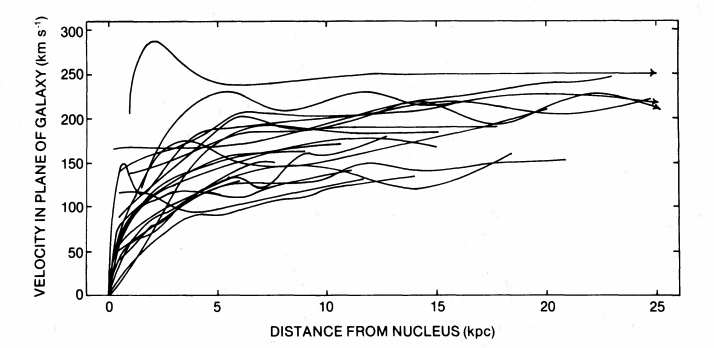
\includegraphics[width=\textwidth]{figures/theory/rot_curves.png}
\caption{Superposition of 21 Sc rotation curves from galaxies with a large range of radii and luminosities. All galaxies have a distinctive flat rotation curve at large radii. Figure from \cite{Rubin1980}.}
\label{fig:curves}
\end{center}
\end{figure}


In order to explain the behavior of galactic rotation curves without dark matter, Milgrom proposed \ac{MOND} in a trio of 1983 papers, \cite{Milgrom1983_1}, \cite{Milgrom1983_2}, \cite{Milgrom1983_3}. Milgrom showed that if Newtonian dynamics was modified from $F = ma$ to $F= ma / a_{0}$, for a $<<$ $a_{0} \approx 1.2 \times 10^{-10} m/s^{2}$ the observed galactic rotation curves could be accounted for without requiring any hidden or dark matter. Milgrom's goal in these first papers describing \ac{MOND} was to present an approximate limit of some as-yet unknown full theory, which he and others went on to develop in the following decades \cite{Bertone2016}. However, theoretical and technological advancements in the fields of cosmology and astronomy have made \ac{MOND} an unsatisfying theory, unable to explain several observed phenomena. Of these phenomena, gravitational lensing and \ac{CMB} are discussed further below.

Big-Bang cosmology had a large success in 1965 with Penzias and Wilsons' observation of the \ac{CMB}. It was in the 1980's however, that cosmology, particle physics, and astronomy became tied together as they are understood today, and dark matter came to refer to an as yet undiscovered particle species and not the cold gas and stars of Zwicky's day \cite{Bertone2016}. The root of this paradigm shift was in the new theory of cosmological inflation \cite{Bertone2016}. Inflation refers to a period of exponential expansion $10^{-36}$ to $10^{-33}$ seconds after Big Bang. Without an inflationary period, fluctuations would be washed out as the universe expanded, leading to a universe devoid of structure. Inflation, however, provides mechanism for quantum fluctuations to be `blown up' and seed the structure observed by the 1982 CfA redshift survey (Figure~\ref{fig:cfa}). Numerical simulations to reproduce the structure seen by the CfA redshift survey benefited from new improvements in processing speed and numerical techniques, and also from the new theory of inflation, which provided a physical reason for initial density perturbations \cite{Bertone2016}. The structure was reproduced only in the presence of gravitationally-interacting dark matter. It is interesting to note here that these cosmological simulations were largely insensitive to any additional, non-gravitational interactions the dark matter had, as long they were sufficiently weak. However, the simulations did require the dark matter to be non-relatistivc or ``cold''. Such dark matter is referred to as \ac{CDM}, and plays a prominent part in the standard cosmology to describe the structure and evolution of our universe at all scales.  

\begin{figure}[htbp]
\begin{center}
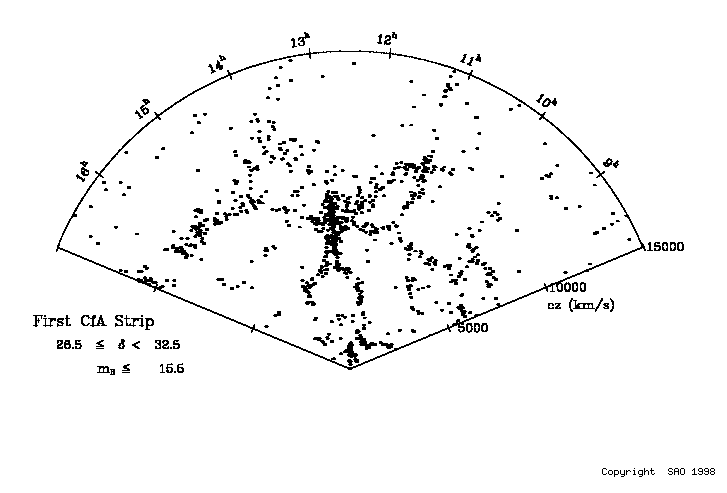
\includegraphics[width=\textwidth]{figures/theory/cfa.png}
\caption{CfA Redshift Survey result showing the distribution of galaxies in a strip on the sky about 6 degrees wide and 130 degrees long. The radial coordinate is redshift, in km/sec, calculated with a Hubble constant of 20km/sec/million ly.}
\label{fig:cfa}
\end{center}
\end{figure}


\section{Evidence for Dark Matter}
The previous section gave an overview of why \ac{CDM} as become, over the last century, the leading paradigm to explain the small and large-scale structure observed in our universe. The following subsections deal with particular pieces of evidence, discussed in detail.

\subsection{Galaxies and Clusters}
Galactic rotation curves were discussed above, as evidence for dark matter halos. Here we further discuss the properties of dark matter halos. An example of a galactic rotation curve of a spiral galaxy showing the presence of an inferred dark matter halo is shown below in Figure~\ref{fig:rot_curve}. Each side of  Figure~\ref{fig:rot_curve} shows the same galaxy, NGC 3198, but fit with a different disk and halo model.  In this particular example from 1985, the authors note their uncertainty about which halo model is the correct one: ``Should one seriously consider the case where the amount of visible matter is negligible with respect to the amount of dark matter [Figure~\ref{fig:rot_curve} (left)]? Or is the maximum disk case [Figure~\ref{fig:rot_curve} (right)] closer to the truth?" \cite{Albada1985}. A decade later, in 1996, Navarro, Frenk and White published a paper describing high-resolution simulations of \ac{CDM}, which could all be fit with a universal dark matter halo profile \cite{Navarro1996}. This formula became known as the \ac{NFW} profile; it is still widely used today, and is the basis for many direct detections experiments, including \ac{LUX}. 

\begin{figure}[htbp]
\begin{center}
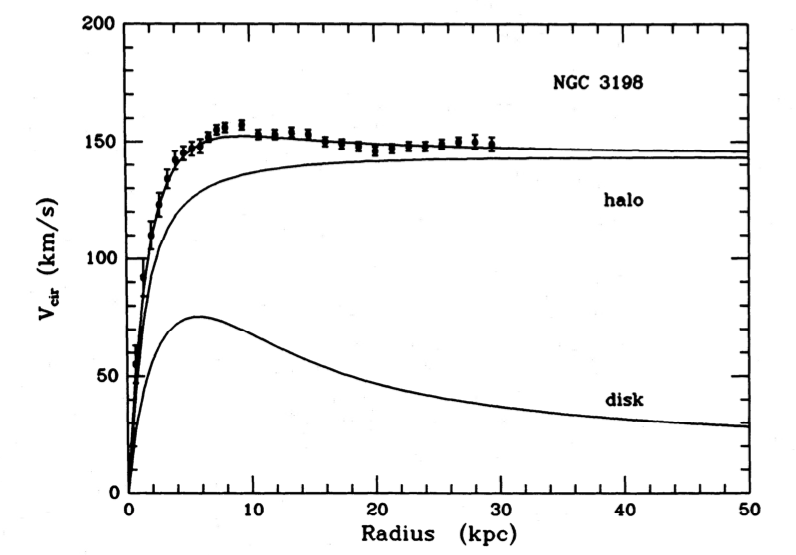
\includegraphics[width=\halffig]{figures/theory/rot_curve2.png}
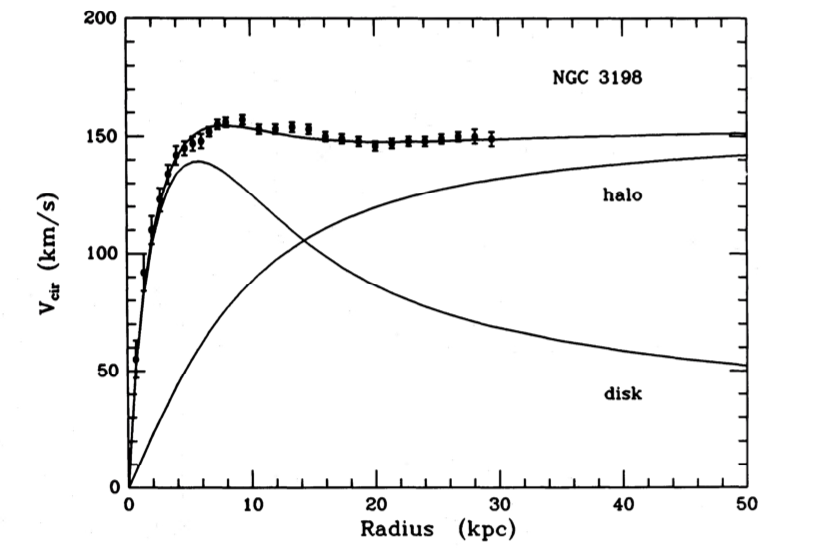
\includegraphics[width=\halffig]{figures/theory/rot_curve1.png}
\caption{Galactic rotation curve from \cite{Albada1985} }
\label{fig:rot_curve}
\end{center}
\end{figure}

The astrophysics community is near unanimous that a galaxies have a dark matter component. Today, research continues into the particular shape of the dark matter profile. While \ac{NFW} is in common use and agrees with many observations, it is not consistent with observations of low surface brightness and dwarf galaxies \cite{DeBlok2001}, \cite{DeBlok2001a}. This known as the core-cusp problem: \ac{NFW} galaxies have an over-density of dark matter at small radius (cuspy), while dwarf galaxies favor flatter density profiles (core). Some argue that such behavior may be a consequence of the nature of dark matter, or that current simulations are not sufficient to properly understand dwarf galaxies \cite{Oman2015}. Others argue that a cusp can be changed to a core via baryonic feedback that arises in simulations of active galactic nuclei \cite{Martizzi2013}. Other current research centers on the globular clusters and stars that orbit the Milky Way. These researchers look for evidence of halo substructure and streams of dark matter from the movements of stars orbiting the Milky Way. Data from the Gaia satellite, launched in 2013, calls into question whether dark matter halos are truly in equilibrium, which has consequences for direct detection experiments, as it would change the expected dark matter recoil spectrum \cite{Herzog-Arbeitman2018} \cite{Necib2018}. In addition to the stars and globular clusters orbiting the Milky Way, there could be clusters of dark matter more dense than the surrounding halo. Telescope data shows evidence for dark matter halo substructure in the Milky Way \cite{Erkal2017}, and simulations expect upcoming data from LSST to further contribute to understanding of Milky Way halo substructure and rule out certain dark matter halo models \cite{Banik2018}.

Galaxy clusters make up some of the strongest direct evidence for dark matter though the method of gravitational lensing. A gravitational lens is created when a massive object is located between a light source and an observer. General relativity requires photons to propagate on the null geodesics of spacetime, meaning the path the light takes from the source will be bent by the distorted space-time of the the massive object. Thus images of background galaxies are distorted by invisible mass along the line of sight from the observer. Being dependent on general relativity, and therefore Newtonian dynamics, the numerous observations of gravitational lensing in large structures strongly disfavor \ac{MOND}. 

There are a few types of gravitational lensing: strong, weak, and microlensing. Weak lensing has been used to observe dark matter in large scale structures (galaxy clusters); the other types of lensing are not treated here. In weak lensing, the light sources are far away from the foreground mass (or the mass is small). Several light sources are required, and the location of mass is statistically reconstructed. The Bullet Cluster (1E0657-558) is one of the most dramatic weak lensing measurements: it is actually the collision of the galaxy cluster 1E0657-56 and smaller cluster (the ``bullet") \cite{Markevitch2001}. The x-ray image of the collision, by the Chandra x-ray observatory, shows the location of the baryonic matter. The baryonic matter suddenly slowed down upon the collision, emitting shock x-rays  \cite{Markevitch2001}. The authors of \cite{Markevitch2001} call it ``a textbook example of a bow shock", indicating the x-ray behavior is well understood. A few years later, Clowe et al. also call the Bullet Cluster ``a direct empirical proof of the existence of dark matter." Their weak lensing observations show the location of the large, invisible (in x-ray and visible light) mass centers of the two clusters to be offset from the location of the baryonic matter at a significance of 8$\sigma$ \cite{Clowe2006}. In the collision, the dark matter halos of the two clusters are expected to pass through each other without slowing down, while the baryonic matter of the two clusters interacts, slowing down. The weak lensing measurement is shown overlaid with the visible and x-ray images in Figure~\ref{fig:bullet}. 

\begin{figure}[htbp]
\begin{center}
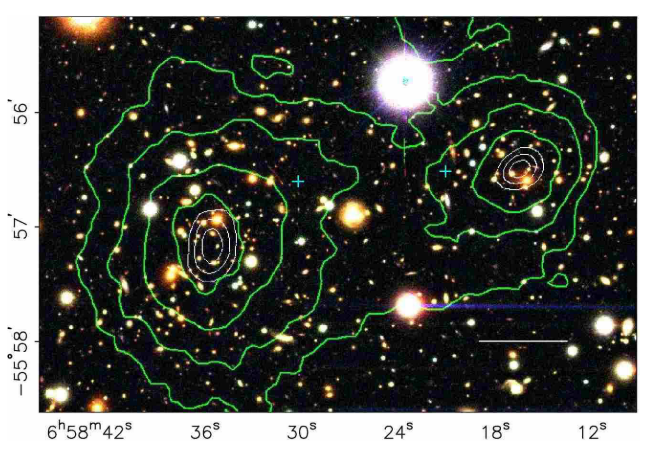
\includegraphics[width=\halffig]{figures/theory/bullet1.png}
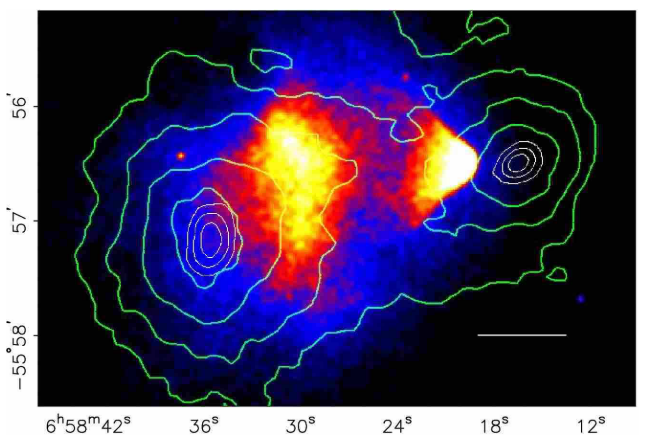
\includegraphics[width=\halffig]{figures/theory/bullet2.png}
\caption{(left) The visible light image from the Magellan telescope of the merging Bullet Cluster overlaid with the weak lensing measurement contours in green, and white 68.3\%, 95.5\%, and 99.7\% confidence levels for the weak lensing peaks. (right) The Chandra x-ray image overlaid with the same weak lensing measurement. Figure from \cite{Clowe2006} }
\label{fig:bullet}
\end{center}
\end{figure}


\subsection{Cosmic Microwave Background}
\label{sec:cmb_dm}
In the thermal history of our universe, the term recombination refers to the epoch when temperatures had cooled enough to allow electrons and protons to combine into hydrogen, leaving photons to propogate freely through the universe. The photons should have decoupled from the matter as a black body peaked at the temperature of recombination,  $\approx$3000~K. The relic radiation from this epoch is visible today as the \ac{CMB}, where the continuing expansion of the universe has redshifted the photons to a temperature of $\approx$2.7~K. The \ac{CMB} photons are also referred to as the light of last scattering, referring to the interaction the photons had with free electrons before the electrons became bound to protons in hydrogen. The temperature of the \ac{CMB} was precisely measured to be 2.7377 $\pm$ 0.0038~K  by the COBE mission, which also confirmed its perfect adherence to a black body spectrum \cite{Smoot1999} (Figure~\ref{fig:cobe}).

\begin{figure}[htbp]
\begin{center}
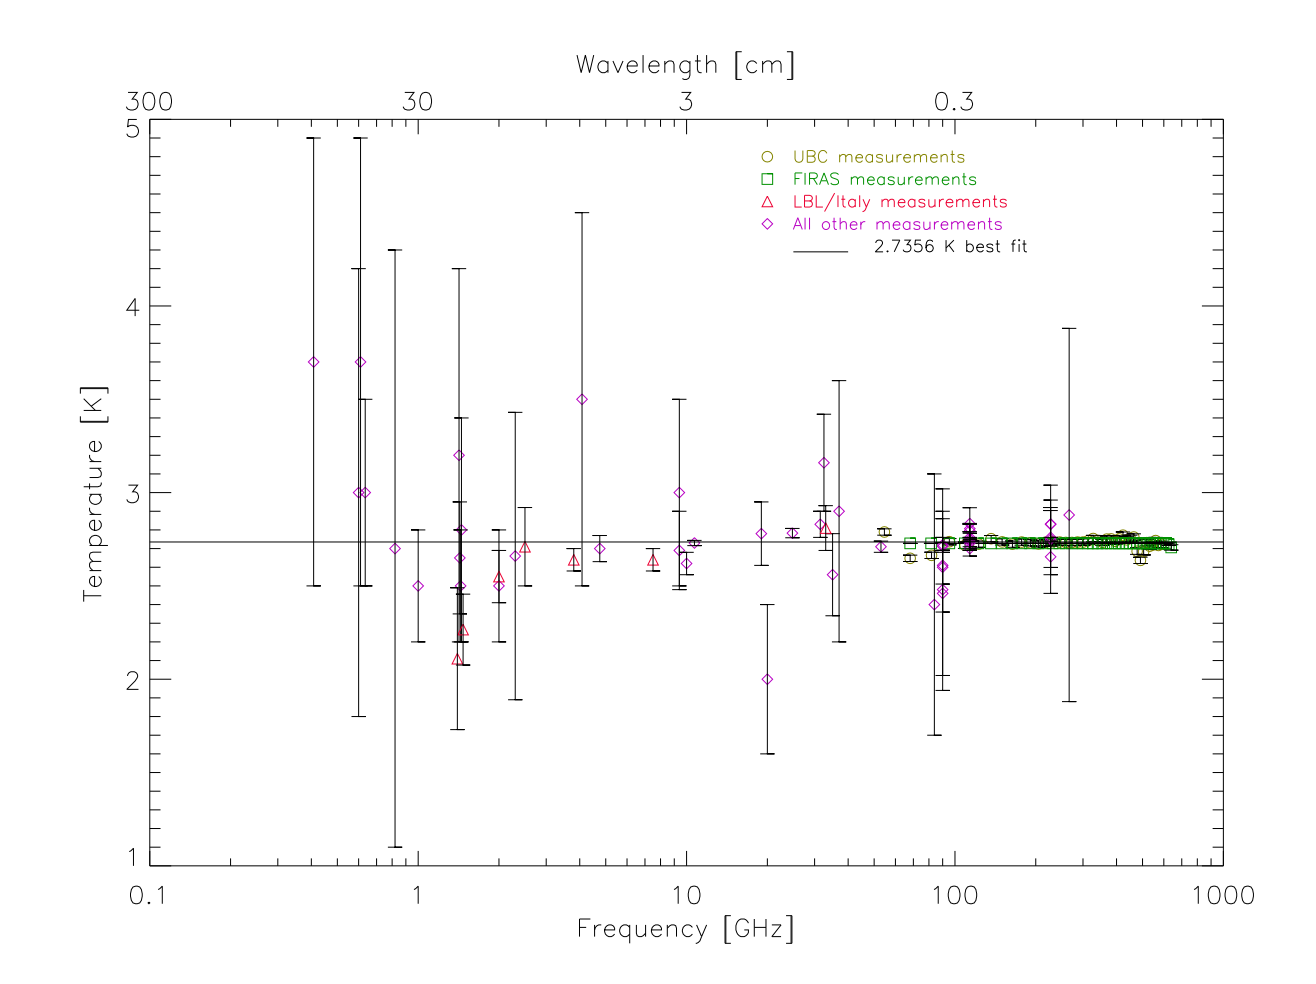
\includegraphics[width=\halffig]{figures/theory/cobe_temp.png}
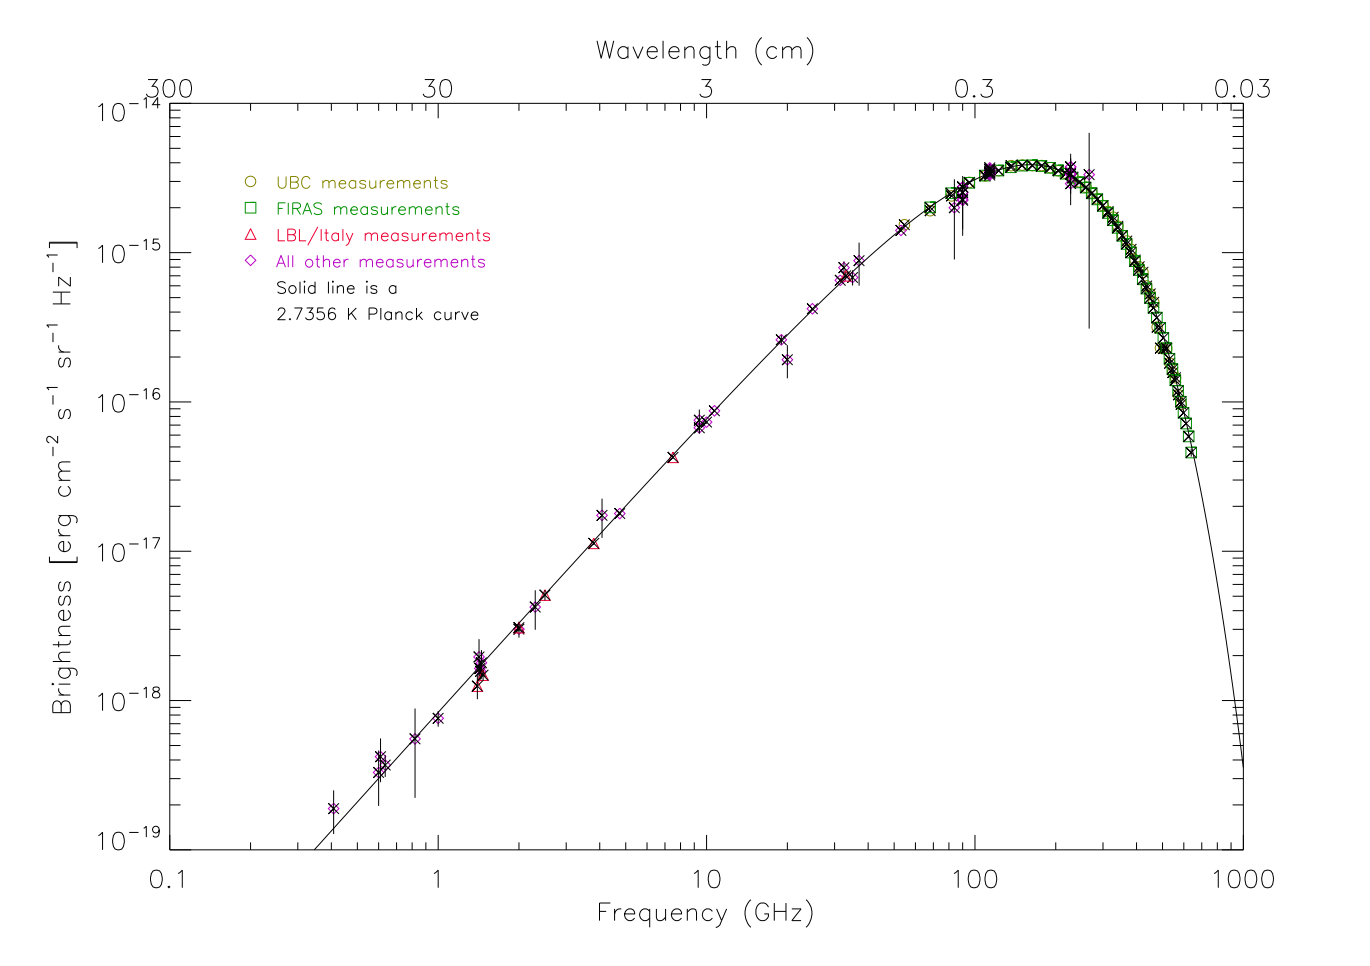
\includegraphics[width=\halffig]{figures/theory/cobe_spectrum.png}
\caption{(left) The FIRAS instrument on the COBE satellite mission measured the \ac{CMB} temperature to be 2.7377 $\pm$ 0.0038~K. (right) The FIRAS instrument also confirmed the perfect Planck black body spectral shape of the \ac{CMB} radiation. Figures from \cite{Smoot1999} }
\label{fig:cobe}
\end{center}
\end{figure}

While the COBE satellite mission's measurements of the \ac{CMB} provided strong support for the Big Bang model of cosmology, it was COBE's discovery of anisotropies in the \ac{CMB} that eventually led to powerful evidence for \ac{CDM}. Since COBE, two more \ac{CMB} satellite missions, WMAP and Planck, have launched and gathered data, each with successively higher spatial and energy resolution. The relative resolutions of COBE, WMAP, and Planck are shown in Figure~\ref{fig:cmb} along with the full Planck \ac{CMB} anisotropy map. The scale of the anisotropy fluctuations represent a scale of  $\pm$~30~$\mu$K; the \ac{CMB} power spectrum remains the most perfect black body spectrum observed in nature. 

\begin{figure}[htbp]
\begin{center}
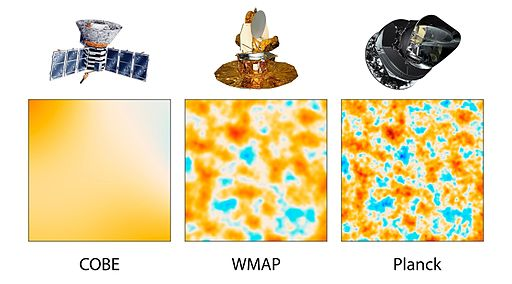
\includegraphics[width=.6\textwidth]{figures/theory/satellites.jpg}
\includegraphics[width=\textwidth]{figures/theory/planck.png}
\caption{(top) The relative spatial resolution of COBE, WMAP, and Planck. Figure courtesy of NASA. (bottom) The Mollweide projection of the Planck 2013 CMB temperature map. The color scale represents fluctuations of $\pm$~30~$\mu$K around a central value of 2.7377~K. Figure courtesy of ESA and the Planck Collaboration. }
\label{fig:cmb}
\end{center}
\end{figure}

The fluctuations $\Delta T(\theta, \phi)$ of the \ac{CMB} map shown in Figure~\ref{fig:cmb} can be decomposed into its basis components via Fourier analysis, where each expansion component is represented by the spherical harmonics, $Y_{lm}$:

\begin{equation}
\label{eq:cmb_fluct}
\Delta T(\theta, \phi) = \sum_{l=2}^{\infty} \sum_{m=-l}^{l} b_{lm} Y_{lm}(\theta, \phi)
\end{equation}

The sum leaves out the $l=0$ (mean) and $l=1$ (dipole Doppler shift caused by movement of the earth) components, which were subtracted from the \ac{CMB} temperature map, leaving only the fluctuations as in Figure~\ref{fig:cmb}. The power spectrum of the temperature fluctuations, which is calculated by squaring Equation~\ref{eq:cmb_fluct}, averaging it over all points that have the same angular separation $\theta$, and performing an integral over all $m$ (because the temperature anisotropies have no preferred direction), encodes all the statistical variation in the \ac{CMB} sky (see, e.g. \cite{Hu2008} for a derivation). The angular correlations of the different multipole moment $l$ are typically extracted from this power spectrum and plotted as function of $l$ and the coefficients $C_{l}$ from the power spectrum. This quantity is referred to as the angular power spectrum and takes the form:

\begin{equation}
D_{l}^{TT} = \frac{ l(l + 1)}{ 2 \pi} C_{l}
\end{equation}
 
where the $TT$ superscript denotes temperature anisotropies (polarization anisotropies, not discussed here, can be parameterized similarly). The latest angular power spectrum from Planck is shown in Figure~\ref{fig:planck_multipole}.

\begin{figure}[htbp]
\begin{center}
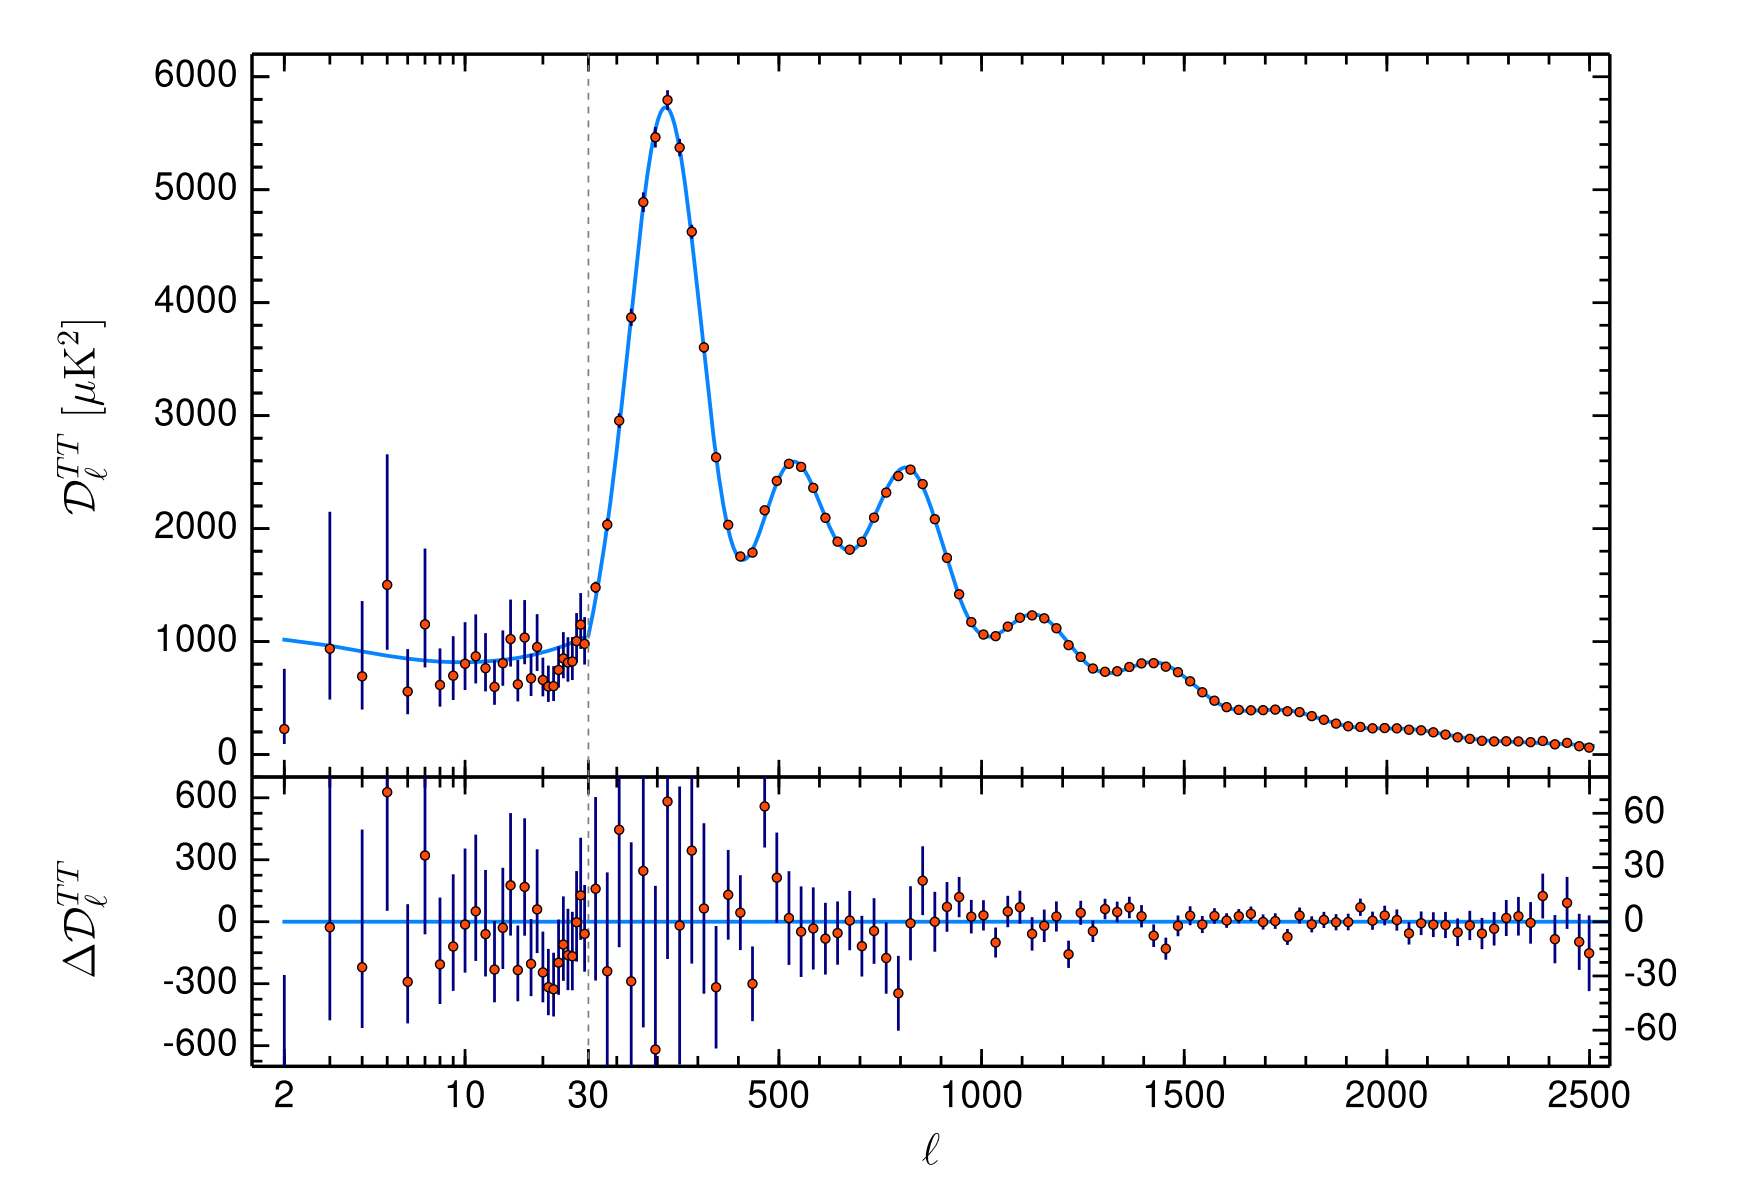
\includegraphics[width=\textwidth]{figures/theory/planck_multipole.png}
\caption{The angular power spectrum from Plank 2018 results  \cite{Planck2018} }
\label{fig:planck_multipole}
\end{center}
\end{figure}

The location and magnitude of peaks in the angular power spectrum (Figure~\ref{fig:planck_multipole}), constrain the curvature, content, and evolution of our universe. The physical interpretation of the \ac{CMB} is as follows: photons from the time of last scattering, newly free to propagate through the universe, carry information about the density fluctuations in the plasma from which they decoupled. The plasma, which was then composed of photons, baryons, and dark matter, behaved as an oscillator driven by gravitational attraction, with a restoring force from the fluid pressure of the plasma. The maxima of the angular power spectrum indicate extrema, overdensities or underdensities, in the plasma. The presence of baryons increases the magnitude of odd peaks relative to even peaks. The physical interpretation of this is that baryons add inertia to the oscillator system, causing an increase in compression (odd) compared to expansion (even) \cite{Hu2008}. The angular power spectrum peaks are sometimes referred to acoustic peaks, as the oscillations that produced them were longitudinal and depended on density, much like sound waves. The presence of dark matter is apparent in the relative heights of the second and third peak in the spectrum. The driving force of the oscillator is total matter content (baryons + dark matter,) which contributes to odd peaks, while baryons contribute characteristically to the even peaks. A third peak that is similar or larger than a second peak indicates that the matter content at the time of recombination was dominated by dark matter. A useful demonstration of the effect of baryons and total matter on the angular power spectrum is shown in Figure~\ref{fig:matter_baryons}.

\begin{figure}[htbp]
\begin{center}
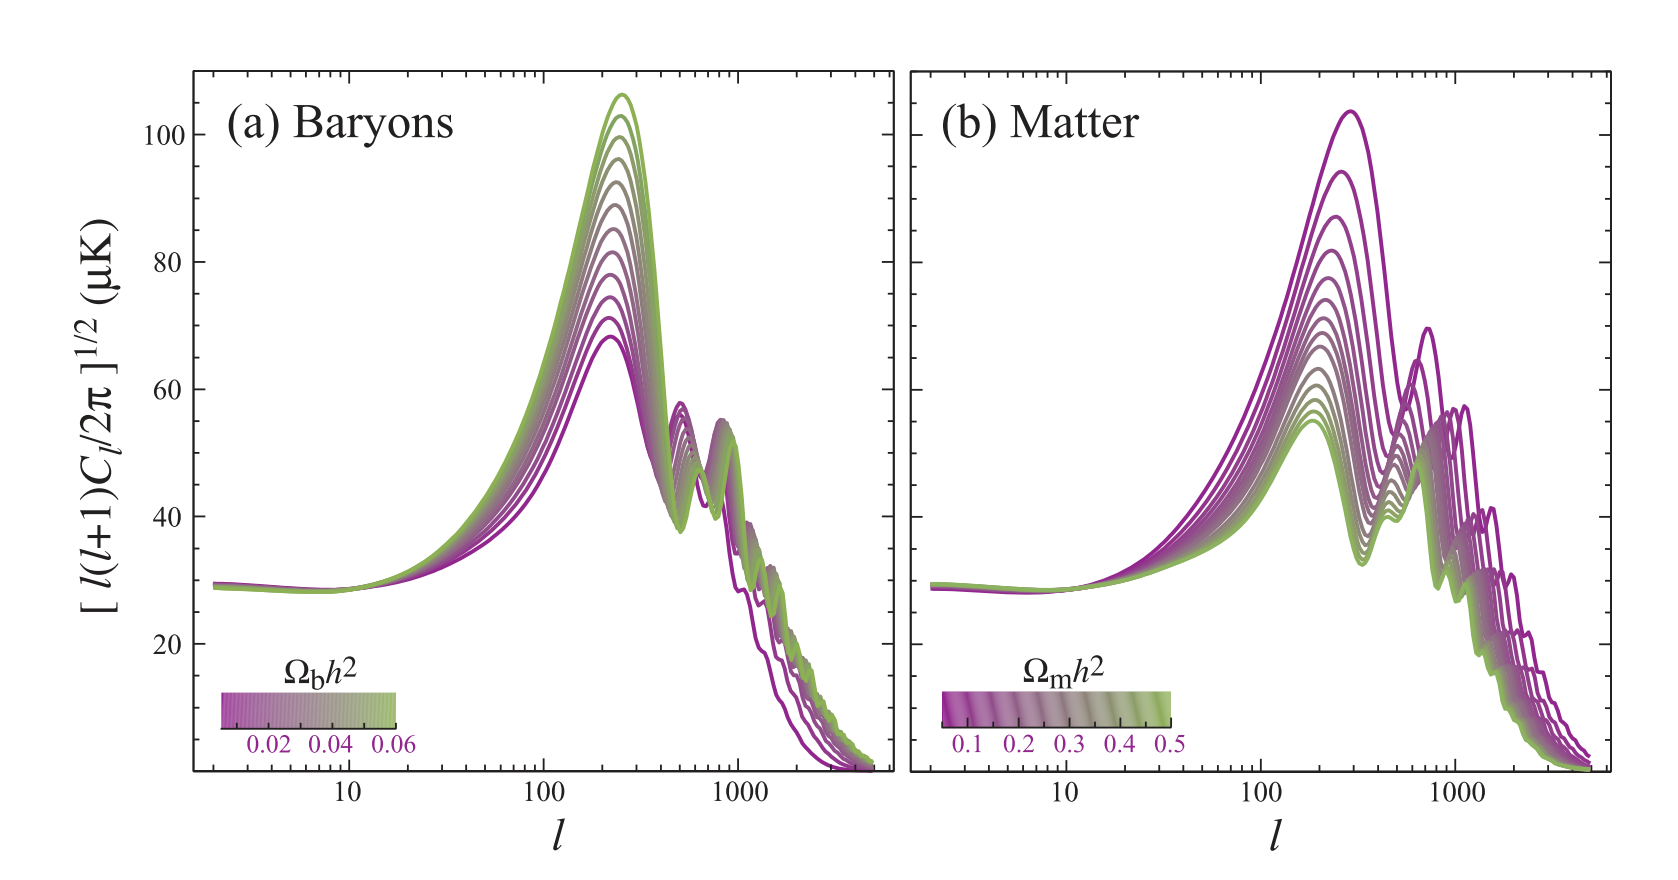
\includegraphics[width=\textwidth]{figures/theory/matter_baryons.png}
\caption{The effect of baryons (left) and total matter (right) on the magnitude and location of \ac{CMB} angular power spectrum peaks.  \cite{Hu2008} }
\label{fig:matter_baryons}
\end{center}
\end{figure}

The measure of the dark matter content and baryon content of today's universe can be extrapolated from fitting the \ac{CMB} angular power spectrum as in Figure~\ref{fig:matter_baryons}. The results from the Planck 2018 angular power spectrum (\cite{Planck2018}) are: 

\begin{equation}
\Omega_{cdm} = 0.2696 \pm 0.0047
\end{equation}

\begin{equation}
\Omega_{b}  = 0.0495 \pm 0.0005 
\end{equation}

Each $\Omega_{x}$ represents the fraction of today's mass-energy density comprised by constituent $x$. These values do not add to one because a large fraction of the mass-energy density of the universe is comprised of dark energy, which we have left discussion of until the next section. However, note that these two values alone measure dark matter to comprise \~84\% of the matter in our universe. 


%; $h$ is the dimensionless version of the Hubble constant, $H_{0}$, which is the dominant source of error in these measurements. The Hubble constant $H_{0}$ is the ratio of the expansion of the universe to its size at $t=t_{0}$ (today). 

\section{Standard Models}
Thus far we have focused only on the astrophysical evidence for particle \ac{CDM}. \ac{CDM} plays a central role in the standard model of cosmology, known as $\Lambda$\ac{CDM} (``Lambda'' - \ac{CDM}). In this section, we briefly summarize the standard models of cosmology and particle physics.

\subsection{The Standard Cosmology}
The standard $\Lambda$\ac{CDM} cosmology is based on the Einstein field equations:

\begin{equation}
R_{\mu \nu} - \frac{1}{2} g_{\mu \nu} R = \frac{8 \pi G}{c^{4}} T_{\mu \nu} + \Lambda g_{\mu\nu}
\end{equation}

where $R_{\mu \nu}$ is the Ricci tensor, $R$ is the Ricci scalar, and $g_{\mu\nu}$ is the metric tensor. $T_{\mu \nu}$ is the stress-energy tensor, $G$ is Newton's gravitational constant, $c$ is the speed of light in vacuum, and $\Lambda$ is the cosmological constant. The equation relates the geometry of space-time (on the left hand side) to the energy content of the universe (on the right hand side). Einstein originally introduced the cosmological constant $\Lambda$ to counteract gravity and produce a steady-state universe. Today, however, we know that the universe is expanding, and the rate of that expansion is accelerating. The second fact, first evidenced by supernova Type Ia measurements \cite{Riess1998} \cite{Perlmutter1998}, is what led to today's understanding of a dark energy. Today, we understand  $\Lambda$ to represent a ``vacuum energy? associated with space-time itself, rather than its matter content. It is the source of the accelerating expansion of the universe, sometimes referred to as ``negative pressure'' or ``gravitational repulsion''. 

The Einstein field equations are solved with the Friedman-Lemaitre-Robertson-Walker metric (not shown, see e.g. \cite{Ryden1999}), which describes the symmetries of the situation: isotropy and homogeneity. The solution yields the Friedman equation, which details how the addition of different energy sources (matter, radiation, dark energy) changes the expansion rate of the universe. The rate of expansion is given by the Hubble constant $H(t)$ (a slight misnomer because it can change over time scales \~ history of our universe). It is defined as $H(t)^{2} \equiv \frac{\dot{a}(t)}{a}(t)$, where $a$ is the so-called scale factor, which is a dimensionless factor that parametrizes the size of the universe. The Friedman equation, given below, delineates how the Hubble constant changes with the energy content $\rho_{tot}$ and curvature $k$ of our universe.

\begin{equation}
H(t)^{2} \equiv \Big( \frac{\dot{a}(t)}{a}(t) \Big) = \frac{8 \pi G}{3} \rho_{tot}(t) - \frac{k}{a(t)^{2}}
\end{equation}

The Friedman equation yields a quantity known as the critical density $\rho_{c}$, which is the density for a flat universe ($k=0$). 

\begin{equation}
\rho_{c}(t) = \frac{ 3 H(t)^{2}}{8 \pi G} 
\end{equation}

A species $x$ is defined has having a fraction of the mass-energy density $\Omega_{x}(t) = \rho_{i}(t) / \rho_{c}(t)$. The individual $\Omega_{x}$ have different time evolutions according to their equation of state (see e.g. \cite{Ryden1999} for complete, pedagogical treatment). After treating equations of state, the Friedman equation can be re-written in a more convenient form: 

\begin{equation}
\label{eq:Lcdm}
\frac{H^{2}}{H_{0}^{2}} = \frac{\Omega_{r, 0}}{a^{4}} + \frac{\Omega_{m, 0}}{a^{3}} + \Omega_{\Lambda, 0} + \frac{( 1 - \Omega_{0})}{a^{2}} 
\end{equation}
  
By measuring the energy content of the universe, we can tell the history and fate of the Universe. This is the core of $\Lambda$\ac{CDM} -- it is essentially a system of equations, which, when solved, describe the history of the universe in terms of a few measurable parameters (e.g $\Omega_{x}$). 

The Planck collaboration fits for a standard, 6 parameter $\Lambda$\ac{CDM}, from the \ac{CMB}. This fit includes some parameters specific to the intricacies \ac{CMB} measurements, as well as the familiar $\Omega_{x}$ density parameters from Equation~\ref{eq:Lcdm}. The 6 fit parameters\footnote{ The density parameters are often reported as $\Omega_{x}h^{2}$ since the main source of error in their measurement comes from the Hubble constant $H_{0}$. $h$ is a dimensionless parameter defined as: $h = H_{0}/ 100~km~s^{-1}~Mpc^{-1}$} are:  $\Omega_{b}h^{2}$, $\Omega_{cdm}h^{2}$, $\tau$, $A_{s}$, $n_{s}$, and $100\theta_{MC}$. Other quantities are derived from these parameters. A summary of the parameters, derived quantities, and their values is given in Table~\ref{tb:planck}. Note that the parameter $A_{s}$ is the amplitude of curvature fluctuations in the \ac{CMB} angular power spectrum (Figure~\ref{fig:planck_multipole}). The effect of baryons and dark matter on the angular power spectrum were discussed in Section~\ref{sec:cmb_dm}. Similarly, dark energy content, curvature, and equation of state of the universe also produce visible effects (see in Figure~\ref{fig:curve_etc}). Namely, dark energy and curvature determine the magnitude of the first peak, and curvature determines peak locations.

\begin{figure}[htbp]
\begin{center}
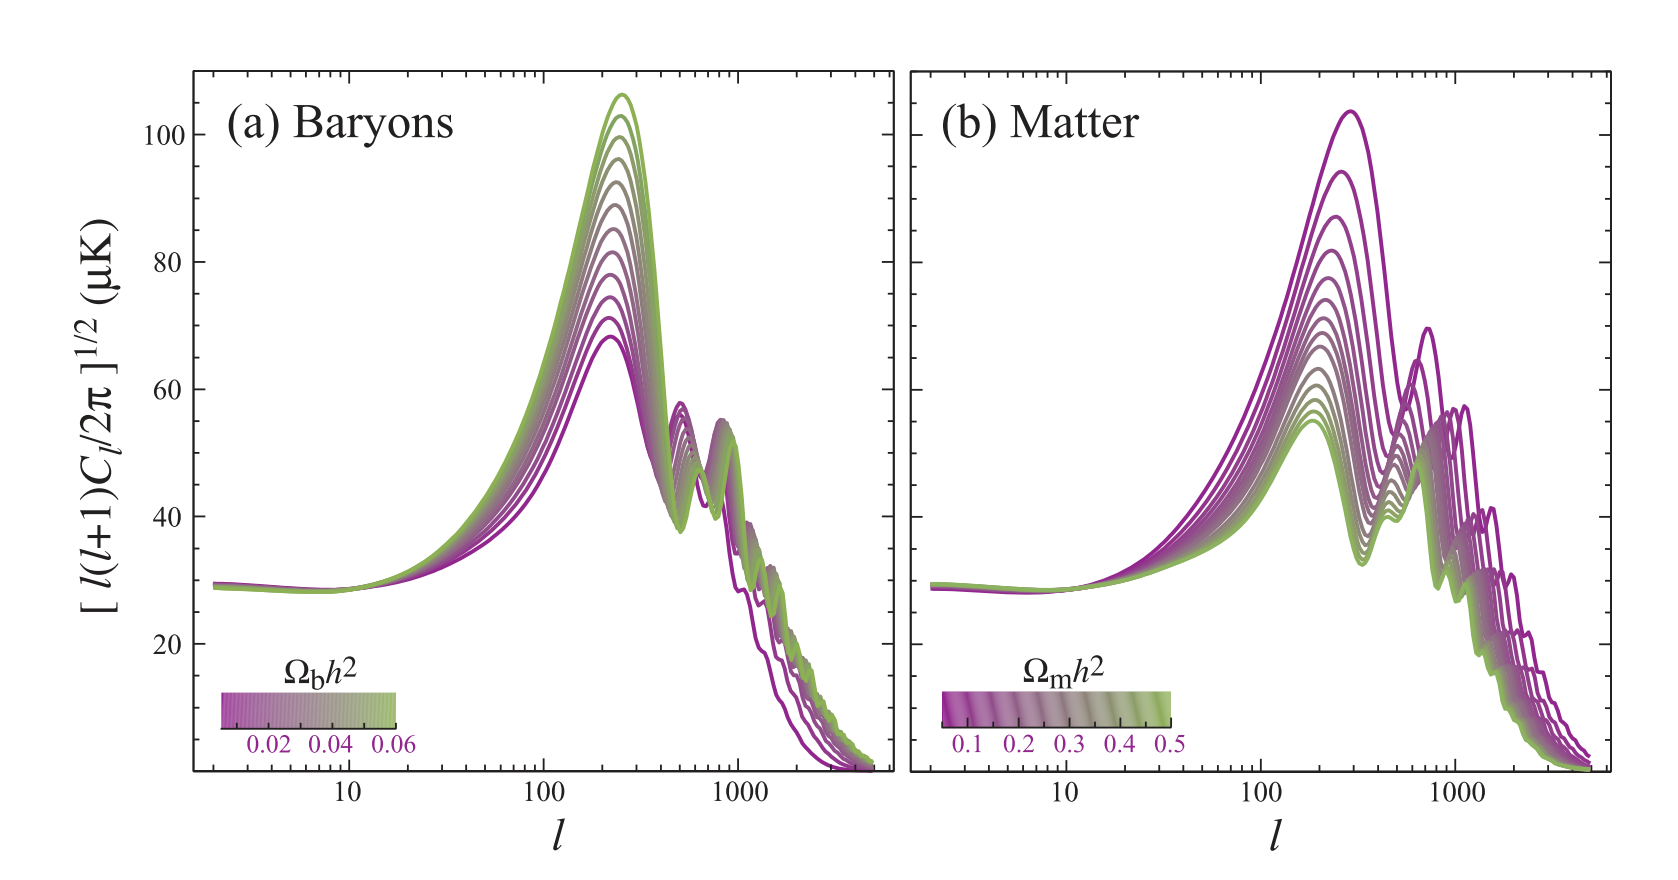
\includegraphics[width=\textwidth]{figures/theory/matter_baryons.png}
\caption{The effect of curvature (left), dark energy (center), and equation of state (right) on the magnitude and location of \ac{CMB} angular power spectrum peaks.  \cite{Hu2008} }
\label{fig:curve_etc.}
\end{center}
\end{figure}


\begin{table}[htp]
\caption{A summary of the fit parameters and derived quantities from Planck's 2018 results \cite{Planck208}.}
\begin{center}
\begin{tabular}{ r l c }
\hline
Fit Parameter & Definition &  Planck TT spectrum \\
\hline
$\Omega_{b}h^{2}$ & baryon density & 0.02212 $\pm$ 0.00022 \\
$\Omega_{cdm}h^{2}$ & CDM density & 0.1206 $\pm$ 0.0021 \\
$100\theta_{MC}$ & angular acoustic scale & 1.04077 $\pm$ 0.00047 \\
$\tau$ & optical depth & 0.0522 $\pm$ 0.0080 \\
$ln(10^{10}A_{s})$ & curvature fluctuations & 3.040 $\pm$ 0.016 \\
$n_{s}$ & spectral index & 0.9626 $\pm$ 0.0057 \\
\hline
Derived Quantity & Definition &  Planck TT spectrum \\
\hline
$\Omega_{b}$ & baryon content & 0.0495 $\pm$ 0.0005 \\
$\Omega_{cdm}$ & CDM content & 0.2696 $\pm$ 0.0047 \\
$\Omega_{m}$  & matter content & 0.321 $\pm$ 0.013 \\
$\Omega_{\Lambda}$  & dark energy content & 0.679 $\pm$ 0.013 \\
$H_{0}$ [km~s$^{-1}$~Mpc$^{-1}$] & Hubble constant & 66.88 $\pm$ 0.92 \\
Age [Gyr]  & age of the universe & 13.830 $\pm$  0.037 \\

\end{tabular}
\end{center}
\label{default}
\end{table}%



\subsection{The Standard Model of Particle Physics}
The \ac{SM} of particle physics describes all the currently known matter particles and force carrier particles, which can also have mass, and which dictate interactions between the matter particles. As of 2012, it also includes a mass generation mechanism from the Higgs boson. The \ac{SM} is formulated using the principles of Quantum Field Theory, where symmetries in the Lagrangian give rise to conserved physical quantities and thereby determine the rules for interactions.

\begin{figure}[htbp]
\begin{center}
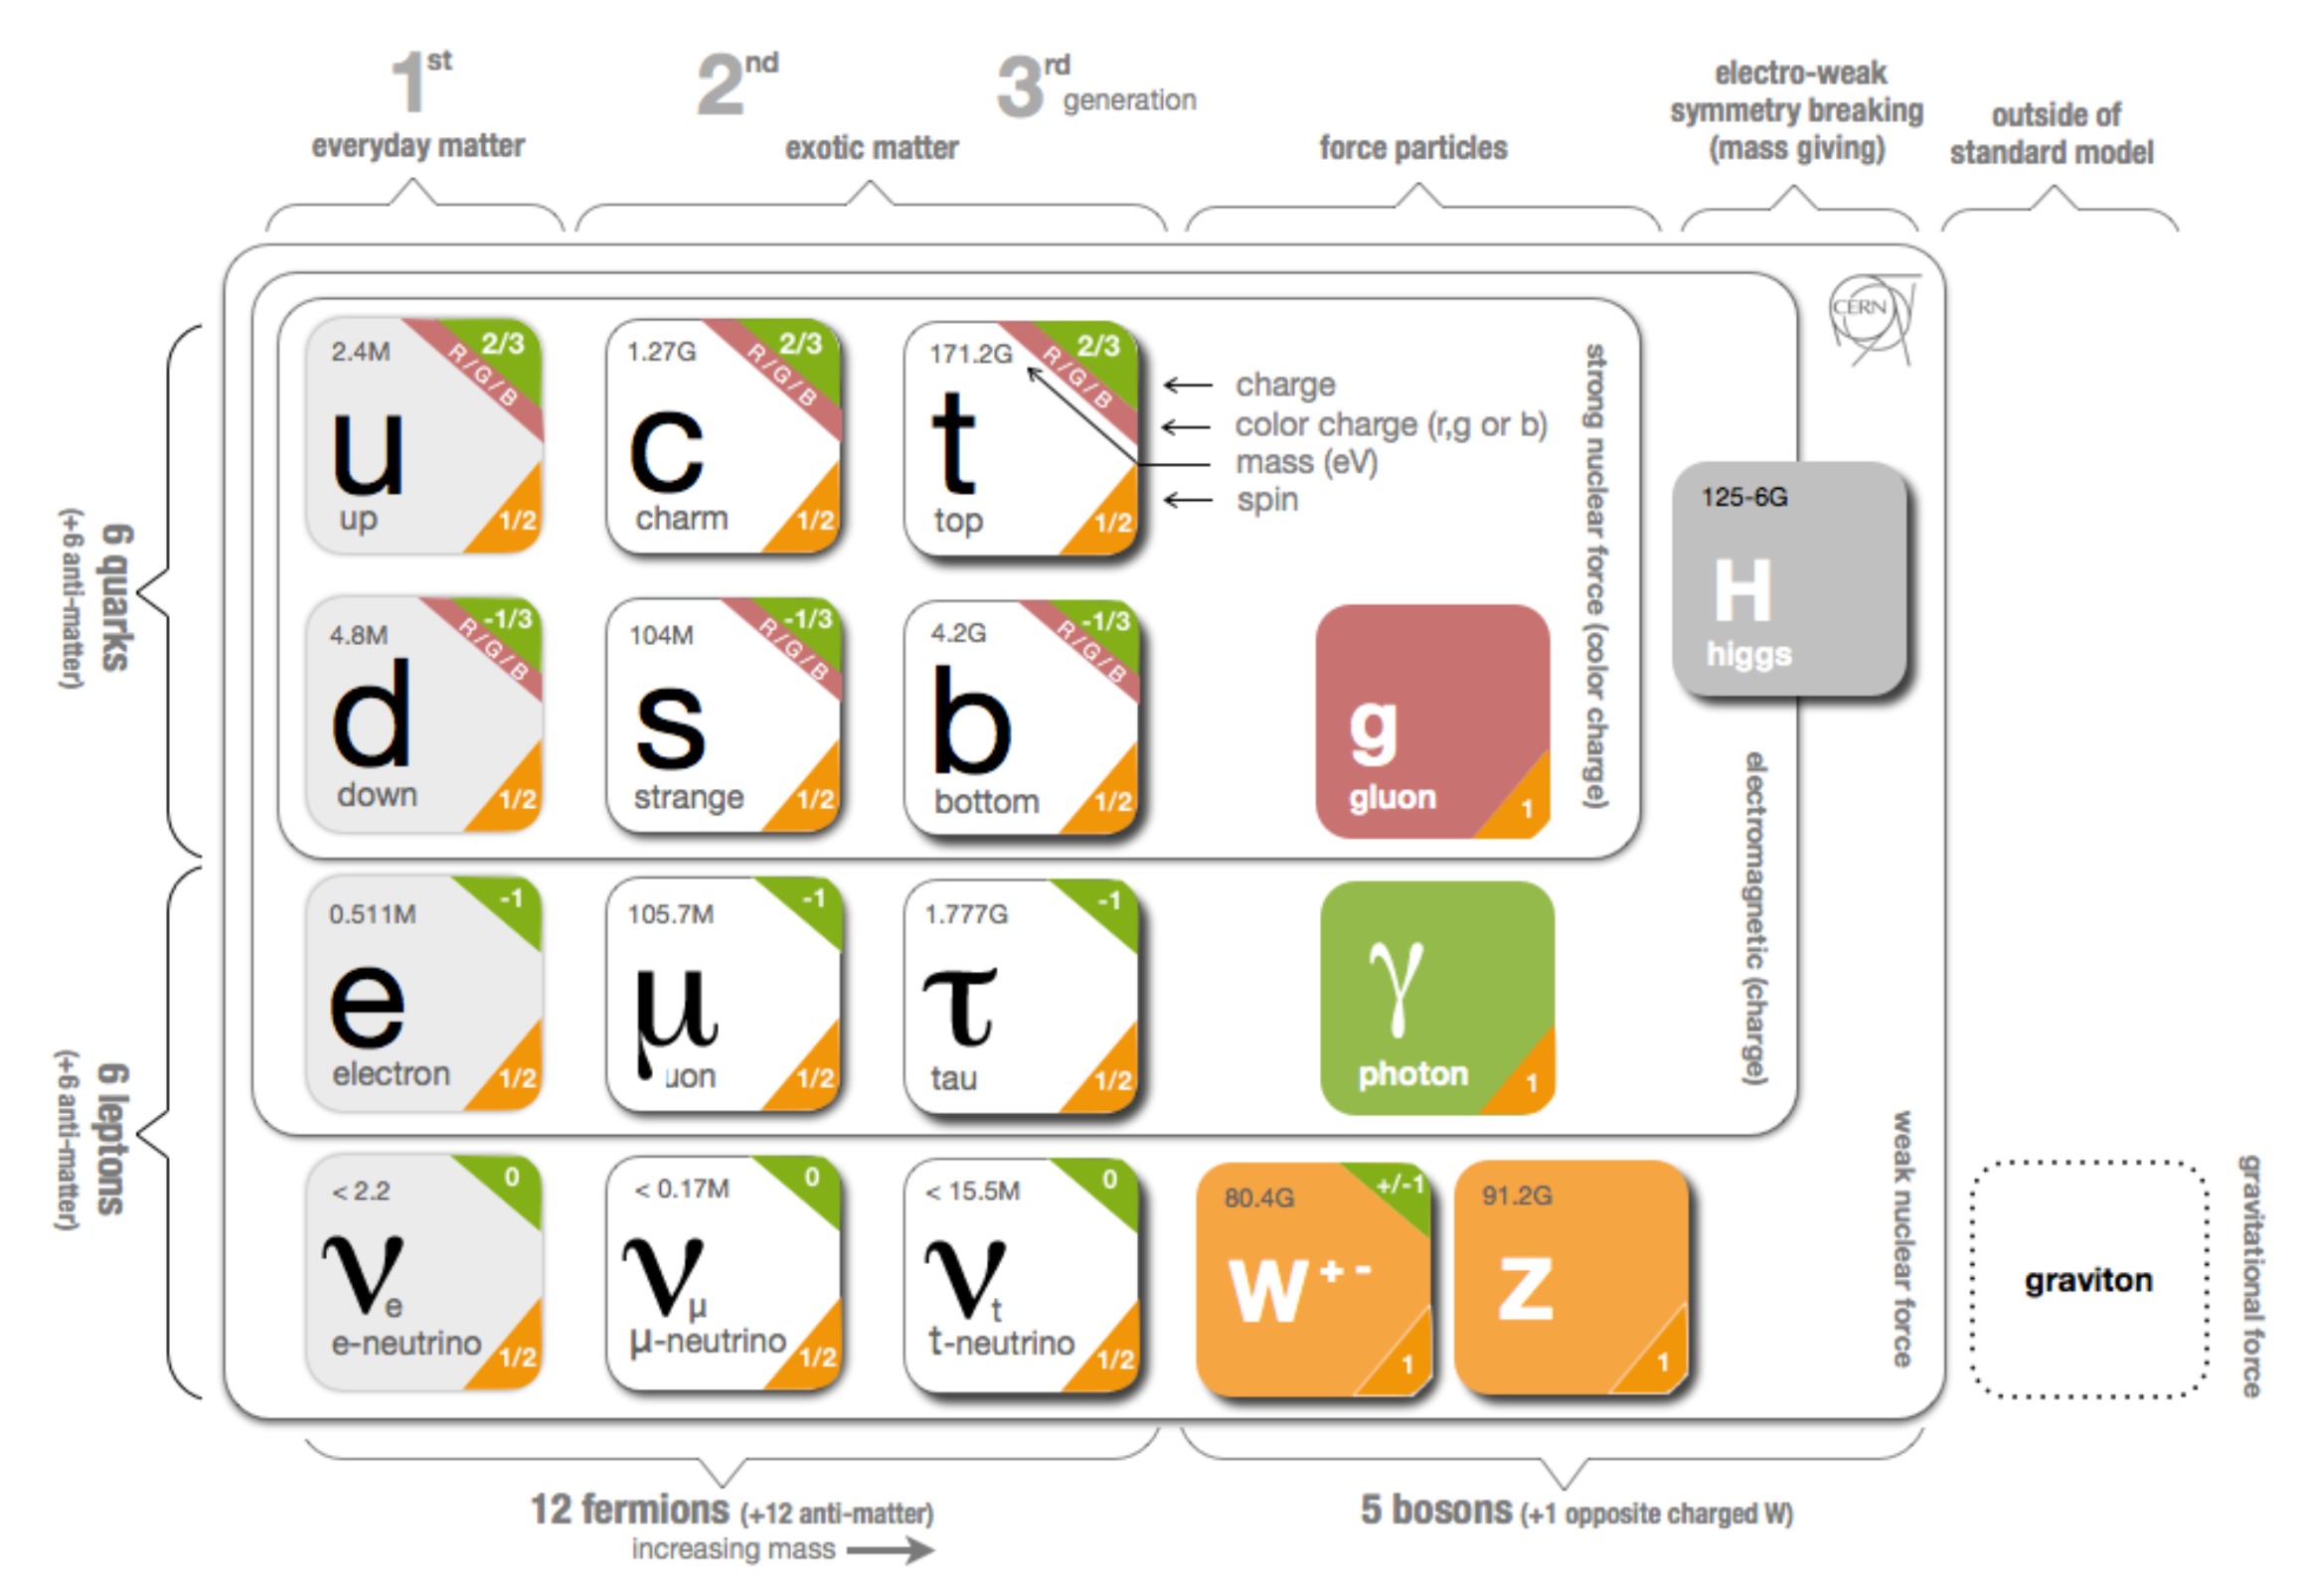
\includegraphics[width=\textwidth]{figures/theory/sm.png}
\caption{The particles that comprise the standard model of particle physics, including names, spins, masses, and charges. It is also indicated which fermions interact with which bosons, e.g. gluons interact with the quarks but not with the leptons. }
\label{fig:sm}
\end{center}
\end{figure}


The known particles of the \ac{SM} are shown in Figure~\ref{fig:sm}, along with a theoretical force carrier for gravity, the graviton. These particles are typically grouped into categories: fermions and bosons. Fermions comprise all the known matter particles and are spin-$\frac{1}{2}$ particles. Each of the fermions in Figure~\ref{fig:sm} has an anti-particle, although it is an open question whether the neutrino is its own anti-particle. The integer-spin bosons, excepting the Higgs boson, which provides a mechanism for giving mass to all the other particles, are the force carriers of the standard model. The spin-1 bosons: the gluon, photon, and $W$ and $Z$ boson, describe three of the four forces known to physics. The gluon mediates the strong force, which governs interactions between quarks, binding them in hadrons (three quark states which make up e.g. protons and neutrons) and mesons (two-quark states such as pions). The photon mediates electromagnetism, governing interactions between particles with electric charge. The $W^{+}$, $W^{-}$, and $Z$ bosons mediate the weak force, which includes phenomena such as beta-decay and neutrino-electron scattering.

It was once proposed that the $Z$ boson could mediate the interaction between \ac{DM} and \ac{SM}, because a \ac{DM} particle that interacts via the weak force fits the \ac{WIMP} paradigm discussed below. However, direct detection experiments have long excluded such scattering cross sections, of $\~10^{-39}~cm^{2}$. Naively, it is possible for neutrinos, which interact weakly and have mass, to be \ac{CDM}. However, neutrinos were relativistic during structure formation so could not perform the role of necessary of \ac{CDM}. Estimates of the density of today's relic neutrinos show that they $\Omega_{v} \approx (1.2 - 2.2) \times 10^{-3} << \Omega_{cdm}$ \cite{Quigg2008}, \cite{Hannestad2004}. The standard model, as it is known today, contains no particles that could be \ac{CDM}. 

\section{Dark Matter Candidates Motivated by Particle Physics}
Cosmology, while providing very precise measurements of the dark matter content of the universe, essentially requires only three things of dark matter candidates: (1) the candidate, $en mass$, must account for the observed $\Omega_{cdm}$, (2) at least 95\% of it is non-relativistic or ``cold'' \cite{something}, (3) it is not strongly self-interacting (``collisionless'') or strongly interacting with baryons. Requirement (1) is fairly loose, as it is possible for multiple different dark matter particles to comprise together $\Omega_{cdm}$, but note that implies the dark matter candidate(s) must be stable on the timescale of the universe. This section briefly summarizes two very different dark matter candidates, which have additional motivation due to open questions from the standard model. 

\subsection{WIMPs and the Hierarchy Problem}
Any system that describes particle interactions today at ``low energy'', should also scale to describe particle interactions at different times (and therefore energies) in the history of our universe, namely immediately after the Big Bang in a time known as the Planck epoch. During the Planck epoch, energies were at the Planck scale of $10^{19}$~GeV, and gravitational interactions become as large as the other forces. Any sound quantum theory should be able to account for gravitational interactions at this energy scale. However, the highest energies described by the \ac{SM} is the known as the electroweak scale, when electromagnetism and the weak force unify. The breaking of the electroweak symmetry is done by the Higgs mechanism, which provides mass. There is a compelling argument that the strong and electroweak forces unify at energies referred to as the \ac{GUT} scale, and that this theory then unifies with gravity at the Planck scale (sometimes called ``Theory of Everything'') \cite{Dimopoulos1991}. The 16 orders of magnitude between the Planck scale and the electroweak scale is known as the Hierarchy Problem; there must be new physics between the electroweak scale and the Planck scale, i.e new particles with $m > m_{Higgs}$ and new symmetries, to properly describe particle interactions during the history of our universe.

In order to solve the Hierarchy Problem, a framework known as \ac{SUSY} was developed. In \ac{SUSY} each \ac{SM} particle has a ``superpartner.'' In general, the superpartners have a spectrum of masses higher than \ac{SM} particles and a symmetry called $R$-parity partitions and limits interactions between \ac{SM} and \ac{SUSY}. The lightest of the \ac{SUSY} particles, called the \ac{LSP}, can be stable. If the \ac{LSP} neutrally charged it is a dark matter candidate.

The \ac{WIMP} paradigm has its roots in the mathematical coincidence called the \ac{WIMP} Miracle. If one assumes a weak-scale coupling and mass for dark matter, it naturally produces the entire $\Omega_{cdm}$ observed today via thermal freezeout. When universe was small and dense with particles, a \ac{WIMP}, $\chi$, would meet its antiparticle $\bar{\chi}$ and annihilate into lighter particles: $\chi \bar{\chi} \longrightarrow l \bar{l}$. The reverse reaction to produce the heavier \ac{WIMP} ($ l \bar{l} \longrightarrow \chi \bar{\chi} $) proceeds as long as the energies of the particle is sufficiently high, i.e. $T > m_{\chi}$. When this condition is met, the number density $n$ of \ac{WIMP}s is at its thermal equilibrium value $n_{eq}$. As the universe expands, the reaction falls out of thermal equilibrium. Both directions of the reaction ($\chi \bar{\chi} \rightleftharpoons l \bar{l}$) are affected: the reverse reaction cannot produce more $\chi$ due to cooling, and the forward reaction stalls because annihilation rate $\Gamma_{A}$ relies on a sufficiently high number density $n$, such that the probability of $\chi$ to meet $\bar{\chi}$ is large. The number density of \ac{WIMP}s become frozen into a relic density that we can observe today when the Hubble expansion rate overcame the annihilation rate:

\begin{equation}
\begin{split}
H(t) &> \Gamma_{A} \\
 &> n_{\chi} \langle \sigma_{A} v \rangle
\end{split}
\end{equation}

where $\langle \sigma_{A} v \rangle$ is the thermally averaged annihilation cross section. The time when $H(t) = \Gamma_{A}$ is referred to as freezeout. Following \cite{Feng2010}, the time evolution of the number density is described by the Boltzmann equation (see Figure~\ref{fig:wimp_miracle} (left) for number density evolution before and after freezeout):

\begin{equation}
\frac{dn}{dt} = -3 H n - \langle \sigma_{A}v \rangle (n^{2} - n_{eq}^{2} )
\end{equation}

This equation must be solved numerically (a more complete analysis can be found in \cite{Lisanti2016}), but making a few assumptions, \cite{Feng2010} finds:

\begin{equation}
\begin{split}
\Omega_{\chi} &\sim \frac{m_{\chi} T_{0}^{3}}{ \rho_{c}} \frac{n_{f}}{T_{f}} \\ %\approx  \frac{20 T_{0}^{3}}{ \rho_{c} M_{Pl} } \langle \sigma_{A}v \rangle^{-1}  \end{equation}
&\propto [\mathrm{constants}] \langle \sigma_{A}v \rangle^{-1} 
\end{split}
\end{equation}

Where $\rho_{c}$ is the critical density, $f$ subscripts refer to freezeout and $0$ subscripts refer to today's values. $\Omega_{\chi}$ then depends only depends on the particular annihilation cross section, which is set by the mass scale $m_{\chi}$:

\begin{equation}
\label{eq:sigmav}
\sigma_{A}v = k \frac{g_{weak}^{4}}{16 \pi^{2}m_{\chi}^{2}} ( \mathrm{1 or} v^{2} ) 
\end{equation}

Where $v^{2}$ is present or absent for S- or P-wave annihilation and $k \sim \frac{1}{2} - 2$ parameterizes the deviation of $g$ from $g_{weak} \approx 0.065$. If the mass of the dark matter particle is in the range $m_{\chi} \sim$ 100~GeV-1~TeV, then $\Omega_{\chi}$ accounts for 100\% of today's observed $\Omega_{cdm}$. This is the \ac{WIMP} miracle: weak-scale particles can account for \textit{all} the dark matter content. Even the \ac{WIMP} mass $m_{\chi}$ deviates from this perfect situation, the particle can still make up a substantial percentage of dark matter (see Figure~\ref{fig:wimp_miracle} (right)),

\begin{figure}[htbp]
\begin{center}
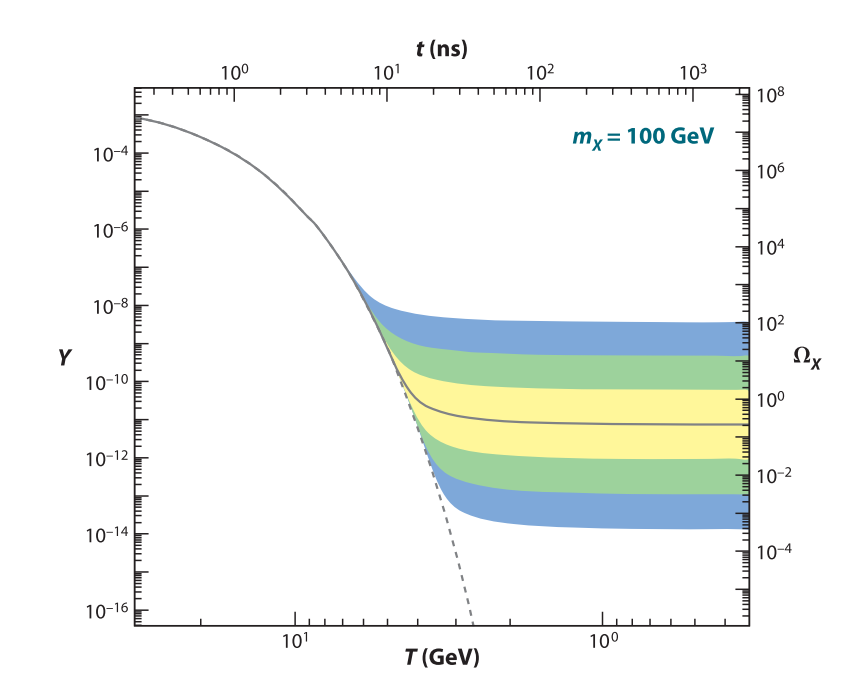
\includegraphics[width=\halffig]{figures/theory/freezeout.png}
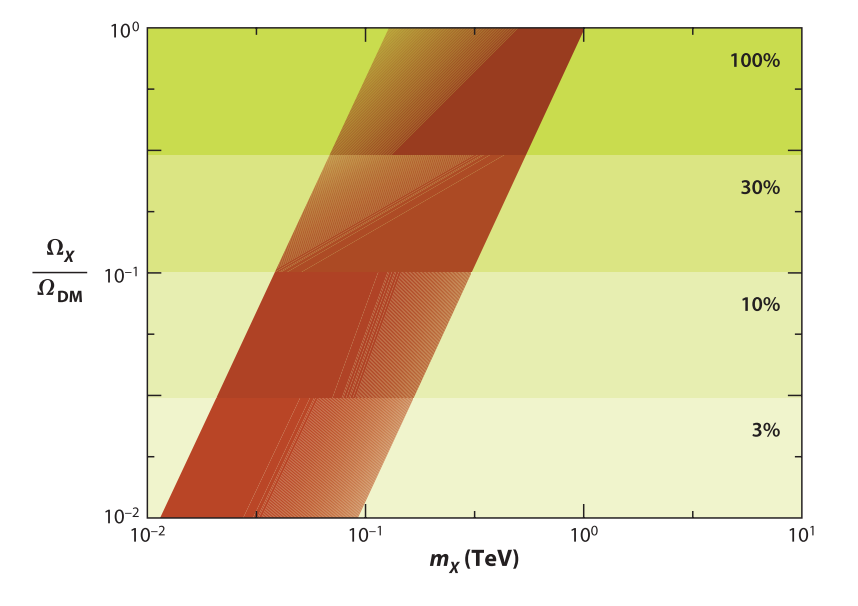
\includegraphics[width=\halffig]{figures/theory/wimp_miracle.png}
\caption{(left) The co-moving number density $Y$ (left y-axis) resulting in the thermal relic density $\Omega_{\chi}$ (right y-axis) for a dark matter particle of mass $m_{\chi}$=100~GeV. The solid black line is the annihilation cross section which yields the correct relic density and bands indicate cross sections that differ by successive factors of 10 from the ``correct'' annihilation cross section (right) A band of natural values for a thermal relic $\chi$ that composes different percentages of the observed dark matter content. The width of the band is set by the deviation of $g$ from $g_{weak}$ in Equation~\ref{eq:sigmav}, Figures from \cite{Feng2010}}
\label{fig:wimp_miracle}
\end{center}
\end{figure}

A particle with the exact mass and weak-scale coupling, i.e the Z-boson has been ruled out by direct detection experiments, but various \ac{SUSY} parameter regions remain. The \ac{LSP} can be a \ac{WIMP}, and thereby it could solve two mysteries of physics: the hierarchy problem, and dark matter. 

\subsection{Axions and the Strong CP Problem}
The \ac{SM} includes a term in the quark sector that should contribute to CP-violating, flavor-conserving, observables that scale with a mixing angle $\theta_{3}$:

\begin{equation}
\mathcal{L} = \theta_{3} \frac{g_{3}^{2}}{32 \pi^{2}} G^{\mu \nu}_{a} \tilde{G}_{a \mu \nu}
\end{equation}

where $g_{3}$ is the gluon coupling constant, $G^{\mu \nu}_{a}$ is the gluon field strength, and $\theta_{3}$ is a dimensionless constant.

This term should produce, for example, an electric dipole moment of the neutron, $d_{e}$. For natural values of $\theta_{3} \sim 1$,  one would expect $d_{e} \sim10^{-16}$~e~cm. However, such a dipole moment has never been observed and current experimental limits constrain $d_{e} < 2.9 \times 10^{-26}$~e~cm \cite{Feng2010}. To account for this, $\theta_{3}$ must be `fine tuned' to $\theta_{3} \longrightarrow \theta_{3}10^{-10}$. This is known as the Strong-CP Problem: we expect CP-violating observables from the \ac{SM}, but instead we find that CP is strongly conserved.

In 1977 Peccei and Quinn proposed a mechanism that solves in the strong CP problem: a new hidden and spontaneously broken global symmetry allows $\theta_{3}$ to be a dynamical value which goes to zero when the symmetry is broken. A spontaneously broken global symmetry generates a Goldstone boson, so there is a new particle with non-zero mass called the axion. Although they are predicted to be light ($\sim \mu$eV to meV), axion production is possible in the early Universe in such a way that they can be \ac{CDM}. Depending on whether the Peccei-Quinn symmetry is broken before or after cosmological inflation, different constrains apply. In either case it is possible for an axion with the appropriate mass to make up all of the $\Omega_{cdm}$ observed today \cite{PDGAxions2017}.



\section{Motivation for LIPs}
Chapter~\ref{ch:lips} of this thesis details a search for \ac{LIP}s, here the theoretical underpinning of such a particle is discussed. 

\section{Experimental Strategies for Detecting Dark Matter}
\subsection{Production}

\subsection{Indirect Detection}

\subsection{Direct Detection}
%*****************************************
%*****************************************
%*****************************************
%*****************************************
%*****************************************
